\section*{Bài 3}

Số $2^{20211309}$ bắt đầu bằng bao nhiêu ?
	
\addcontentsline{toc}{section}{Bài 3}

\begin{center}
    \textbf{\underline{Bài làm:}}
\end{center}

Giả sử cho số ban đầu là $n^k$, với $n, k \in \mathbb{Z}$. Tìm chữ số bắt đầu của $n^k$. Nếu giá trị của $n^k$ quá lớn, vượt quá giá trị tính toán của máy tính thì ta cần tìm một cách khác để tìm chữ số bắt đầu của $n^k$.

Ta sẽ biểu diễn số $n^{k}$ dưới dạng $x \cftdot 10^\alpha$, với $x \in \mathbb{R}, \alpha \in \mathbb{Z}$. Khi đó việc tính toán giá trị của biểu thức $x \cftdot 10^\alpha$ chỉ là dịch chuyển dấu thập phân của số $x$ sang bên phải $\alpha$ chữ số (trường hợp nếu hết số, không thể dịch chuyển được nữa thì ta chỉ thêm số 0 vào bên phải số lúc trước). Việc làm này không thay đổi chữ số bắt đầu của số ta cần tính.

Ta có công thức chuyển đổi như sau:
$$n^k = 10^{\log_{10} \left( n^k \right)} = 10^{k \log_{10}n}$$
Sau đó, ta biến đổi số mũ $k \log_{10}n$ thành một tổng gồm 2 số thực và số nguyên nào đó. Cách đơn giản nhất là ta biểu diễn:
$$k \log_{10}n = \text{truncate}(k \log_{10}n) + \left( k \log_{10}n - \text{truncate}(k \log_{10}n) \right)$$
trong đó, truncate() là phép lấy phần nguyên của một số.

Như vậy:
\begin{align*}
10^{k \log_{10}n} & = 10^{\text{truncate}(k \log_{10}n) + \left( k \log_{10}n - \text{truncate}(k \log_{10}n \right)} \\
                  & = 10^{\text{truncate}\left( k \log_{10}n \right)} \cftdot 10^{k \log_{10}n - \text{truncate}(k \log_{10}n)}
\end{align*}

Quay lại với bài toán ở trên, ta cần tìm chữ số bắt đầu của số $2^{20211309}$.

Ta có: $\log_{10}2^{20211309} = 20211309\log_{10}2 = 6084210.2606...$

Suy ra: $2^{20211309} = 10^{6084210.2606...} = 10^{6084210} \cftdot 10^{0.2606...} \approx (1.8223...) \cftdot 10^{6084210}$ (chỉ cho kết quả xấp xỉ, một vài số đầu của số $x$ và số ban đầu có thể giống nhau, còn các chữ số còn lại có thể khác nhau).

Vậy ta có chữ số bắt đầu của số $2^{20211309}$ là số 1.

\textbf{Tính toán trong Maple:}

Ta thử nhập số $2^{20211309}$ vào trong Maple thì được kết quả:

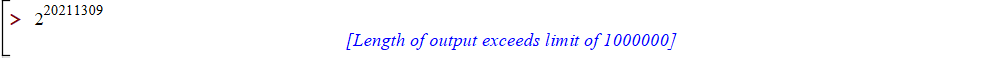
\includegraphics[width=1.0\textwidth]{bai3_maple.PNG}

Vì giá trị của $2^{20211309}$ quá lớn nên Maple không hiển thị ra kết quả tính toán cho ta. Do đó, ta sẽ giải quyết bài toán bằng cách sử dụng ý tưởng ở trên. Ta sẽ định nghĩa thủ tục (procedure) $FindFirstDigit$ như trong hình bên dưới. Sau đó, ta chạy thử với $n = 2$ và $k = 20211309$ và được kết quả là số 1.

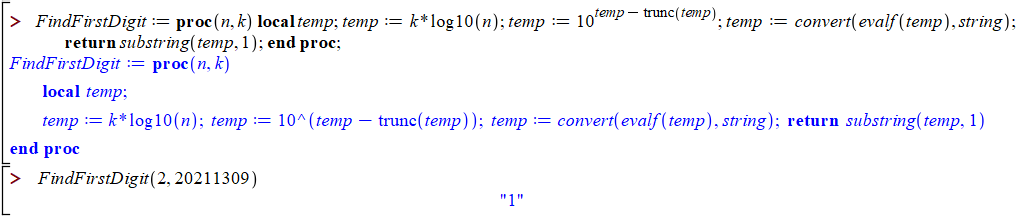
\includegraphics[width=1.0\textwidth]{bai3_maple1.PNG}

Ta có thể kiểm tra lại kết quả tính toán sử dụng \textbf{WolframAlpha}:

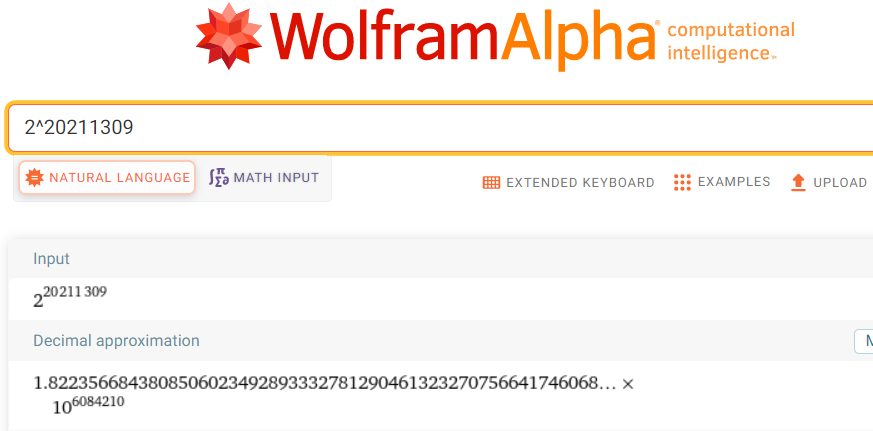
\includegraphics[width=1.0\textwidth]{bai3_wolfram_alpha.PNG}

\textbf{WolframAlpha} vẫn hiển thị kết quả chữ số bắt đầu của số $2^{20211309}$ là số 1.
	
\clearpage